\section{Method}

\subsection{Observation Routing Contract}

GDOR-SLAM extends the RGB-D path of Photo-SLAM~\cite{huai2024photoSLAM}, with an ORB-SLAM3 frontend~\cite{campos2021orbslam3} and a 3DGS mapping backend~\cite{kerbl20233dgaussian}.
All masks below are binary and defined per pixel $\mathbf{x}$.
Let $M_t^{\mathrm{sem}}=1$ denote semantic exclusion and $M_t^{\mathrm{flow}}=1$ denote residual-motion exclusion.
Their union and its morphological closing are
\begin{equation}
D_t^{\mathrm{raw}}=M_t^{\mathrm{sem}}\lor M_t^{\mathrm{flow}},\qquad
\bar D_t=\operatorname{Close}(D_t^{\mathrm{raw}}).
\label{eq:raw-dynamic}
\end{equation}
The claim-bearing configuration routes two different signals: a binary support mask $S_t^{\mathrm{track}}$ to ORB extraction and current-frame tracking, and a float weight $W_t^{\mathrm{map}}$ to persistent ORB/Gaussian mapping.
The conservative mapping route is fixed as
\begin{equation}
W_t^{\mathrm{map}}(\mathbf{x})=1-\bar D_t(\mathbf{x}).
\label{eq:mapping-weight}
\end{equation}
Thus, a tracking decision can recover support without clearing the persistent mapping exclusion.

\begin{figure*}[t]
  \centering
  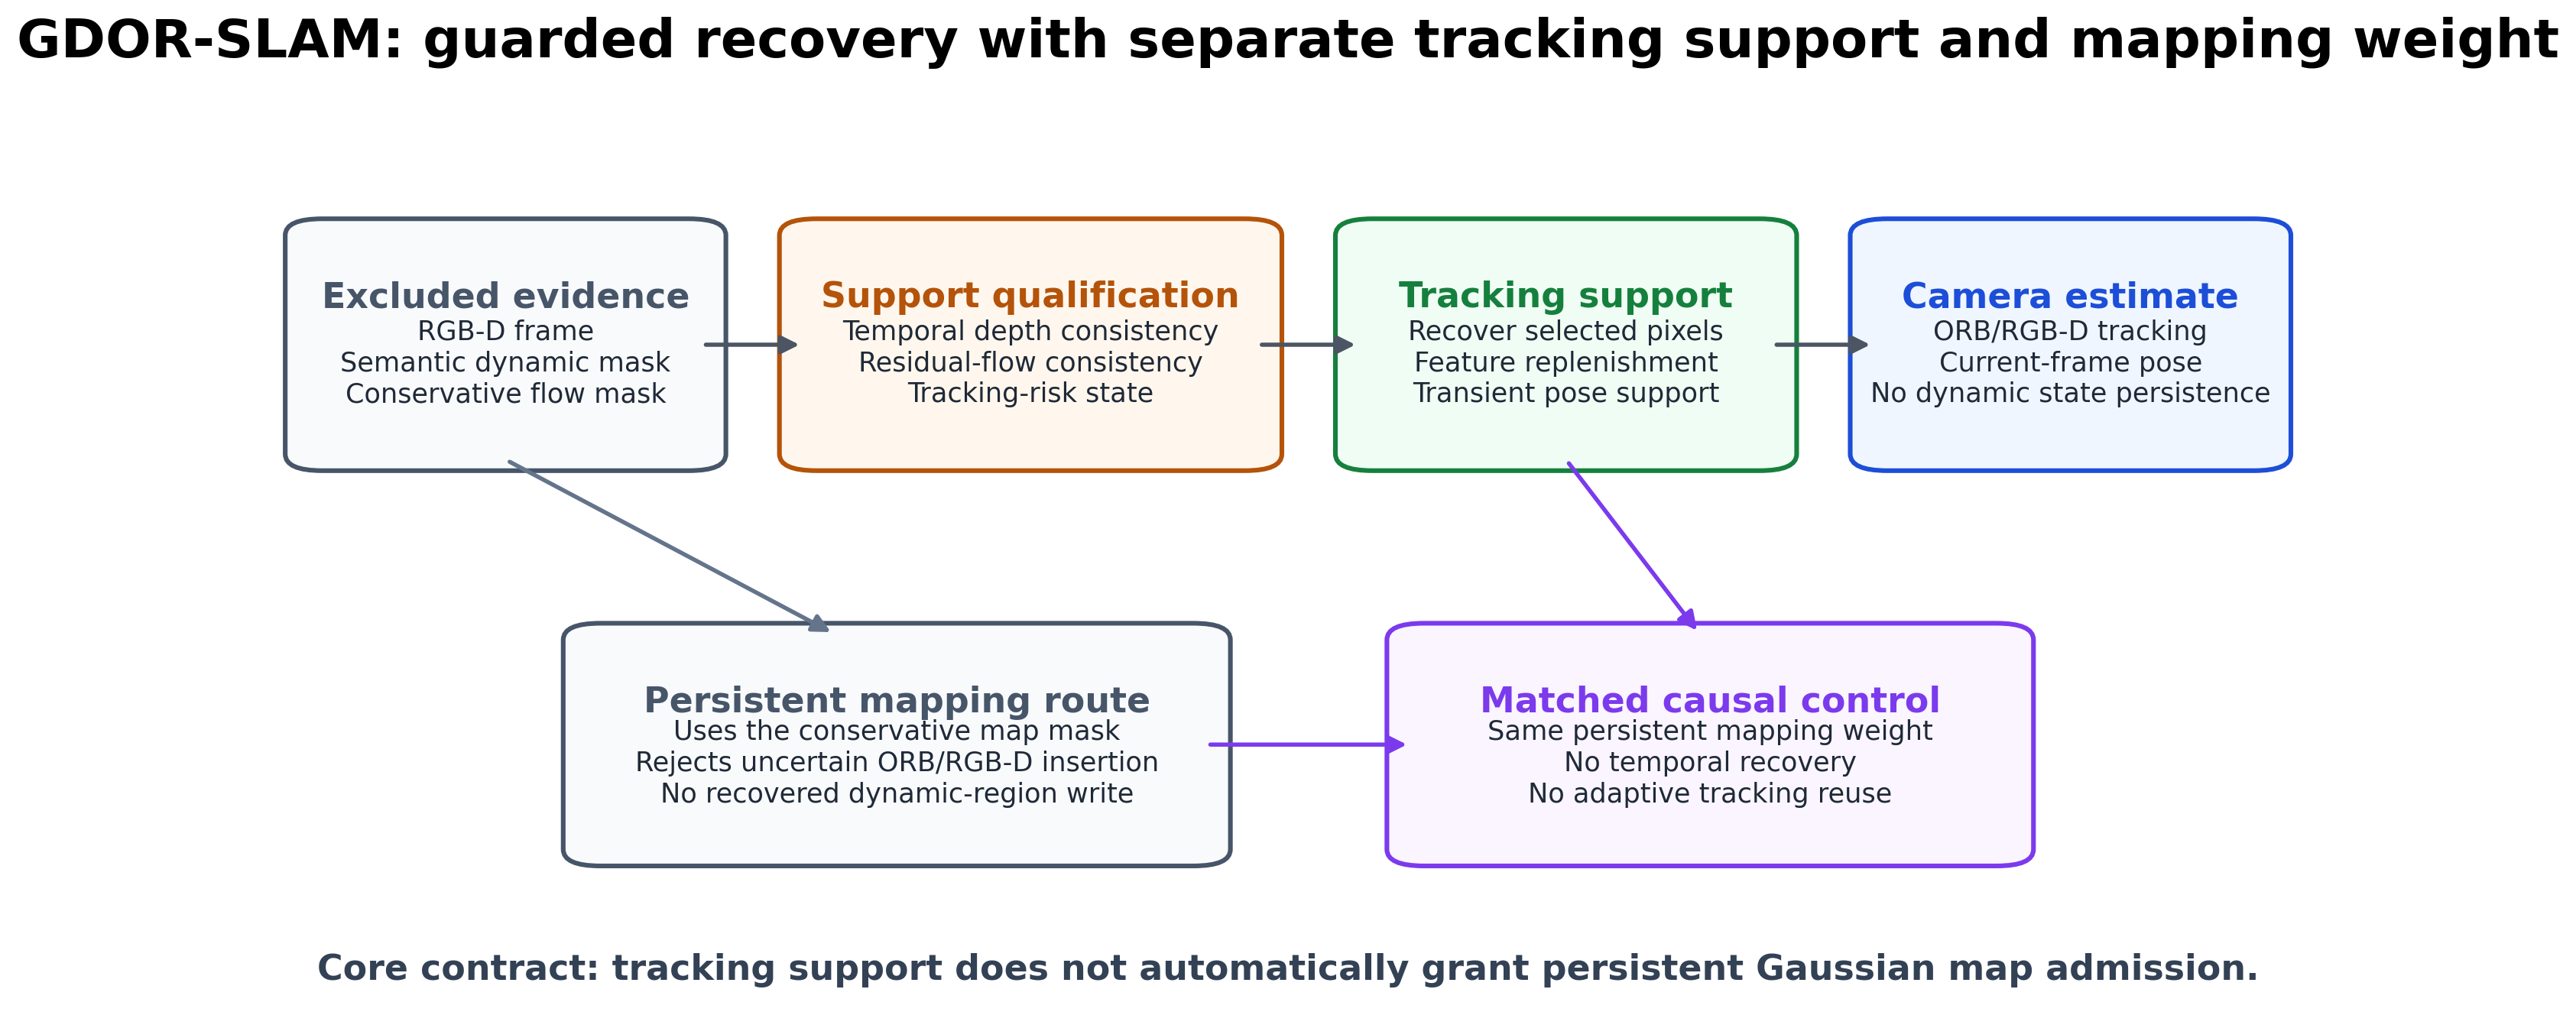
\includegraphics[width=0.96\linewidth]{figures/fig2_method_schematic.png}
  \caption{GDOR-SLAM separates support qualification, transient tracking support, and persistent mapping weight. The matched no-track-reuse control uses the same persistent weight as GDOR but disables temporal recovery and adaptive tracking reuse.}
  \label{fig:method}
\end{figure*}

\subsection{Residual-Flow and Temporal-Depth Evidence}

A semantic prior marks classes that may move.
Forward--backward Lucas--Kanade tracks~\cite{lucas1981optical} are sampled on an image grid; tracks with more than 1.5 pixels of round-trip error are discarded.
A partial affine model is fitted by RANSAC on semantic-static support, while a fundamental-matrix check requires at least six model correspondences and at least 60\% epipolar inliers.
If either model is invalid, flow-based recovery fails closed.
Otherwise, residuals unexplained by the affine model form $M_t^{\mathrm{flow}}$, and the full-frame residual mask plus a safety neighborhood forms the recovery veto $G_t$.

Let $z_t$, $z_t^r$, and $b_{t-1}$ be observed, rendered, and historical background depths.
For valid inputs, the temporal prior is
\begin{equation}
b_t(\mathbf{x})=
\frac{w_h I_h b_{t-1}(\mathbf{x})+w_r I_r z_t^r(\mathbf{x})}
{w_h I_h+w_r I_r},
\label{eq:background-depth}
\end{equation}
where $I_h$ and $I_r$ indicate valid historical and rendered depth.
Depth consistency is accepted when rendered support is valid and at least $K$ valid observations in a local neighborhood $\mathcal N(\mathbf{x})$ satisfy
\begin{equation}
\mathcal C_t^{\mathrm{depth}}(\mathbf{x})=
\left[
\sum_{\mathbf{y}\in\mathcal N(\mathbf{x})}
\mathbf{1}\!\left(|z_t(\mathbf{y})-b_t(\mathbf{x})|<\tau_d\right)
\ge K
\right].
\label{eq:depth-consistency}
\end{equation}

\subsection{Guarded Support Qualification}

A raw-excluded pixel is eligible for tracking recovery only when every required signal is valid:
\begin{equation}
R_t^{\mathrm{elig}}(\mathbf{x}) =
D_t^{\mathrm{raw}}(\mathbf{x})
\land \mathcal{C}_t^{\mathrm{depth}}(\mathbf{x})
\land \neg G_t(\mathbf{x}).
\label{eq:recovery}
\end{equation}
After the same morphological refinement used by the frontend, the tracking support is
\begin{equation}
S_t^{\mathrm{track}}(\mathbf{x}) =
\neg\operatorname{Close}\!\left(
D_t^{\mathrm{raw}}\land\neg R_t^{\mathrm{elig}}
\right)(\mathbf{x}),
\label{eq:tracking-support}
\end{equation}
and the support actually recovered after refinement is
$R_t=D_t^{\mathrm{raw}}\land S_t^{\mathrm{track}}$.
Invalid depth, insufficient rendered support, or an invalid motion model sets $R_t^{\mathrm{elig}}=0$ and returns the conservative raw-mask behavior.

\subsection{Risk-Conditioned Tracking Recovery}

Recovery is useful only when the tracker needs additional support.
GDOR therefore conditions feature replenishment on the previous optimized inlier count.
During a tracking-risk window, the FAST threshold is temporarily relaxed and qualified pixels can participate in feature extraction and current-frame pose estimation.
The relaxation persists for a short fixed hold interval to avoid frame-to-frame switching.
Outside these windows, the system remains close to semantic hard exclusion.

The default Guarded configuration uses residual-flow protection, temporal-depth recovery, and risk-conditioned feature replenishment.
The Strict configuration adds an RGB-D camera-guided flow model and tighter model-quality gates.
Strict is retained as a stronger-intervention control, not as the proposed default, because stronger recovery is not uniformly more stable in the broader TUM/Bonn protocol.

\subsection{Tracking--Mapping Decoupling and Matched Control}

Recovered observations are transient.
They may support current-frame ORB extraction and pose optimization, but the mapping route continues to use Eq.~\eqref{eq:mapping-weight} for Gaussian loss weighting, RGB-D densification, and MapPoint-to-Gaussian admission.
The implemented routing cases are summarized compactly as
\begin{equation}
\begin{array}{c|cc}
\text{configuration} & S_t^{\mathrm{track}} & W_t^{\mathrm{map}} \\
\hline
\text{Semantic} & 1-\operatorname{Close}(M_t^{\mathrm{sem}}) & 1\ \text{(default)} \\
\text{Matched} & 1-\bar D_t & 1-\bar D_t \\
\text{GDOR/Strict} & \text{Eq.~\eqref{eq:tracking-support}} & 1-\bar D_t
\end{array}
\label{eq:routing-matrix}
\end{equation}
The Semantic row has no supplied static weight, so the mapper reports its default unit support; this does not mean that the semantic tracking mask contains no exclusions.

The release audits the exact overlap
\begin{equation}
L_t=R_t\land\mathbf{1}[W_t^{\mathrm{map}}\ge0.5].
\label{eq:leak-audit}
\end{equation}
For the claim-bearing routing, the intended invariant is $|L_t|=0$.
The counter is diagnostic and does not modify either route.
Persistent ORB MapPoints are additionally checked against keyframe static weights, while Gaussian training and RGB-D densification consume the same bound weight.

To isolate tracking-side recovery from the raw-mask route, the map-matched no-track-reuse control uses the same $W_t^{\mathrm{map}}=1-\bar D_t$ as GDOR, uses $1-\bar D_t$ directly for tracking, and disables temporal recovery and adaptive feature replenishment.
The GDOR--Matched comparison therefore tests qualified tracking reuse on top of the same persistent mapping weight; it is not a comparison between two Gaussian-admission masks.

\subsection{Implementation Details}

The frozen Guarded configuration applies semantic inference on every frame after a 50-frame system warmup and starts temporal background refinement after five frames.
Lucas--Kanade tracking uses a $21\times21$ window, three pyramid levels, and an 8-pixel sampling grid.
The dominant-flow residual threshold is 1.5 pixels.
Temporal depth combines rendered and historical background estimates with weights 0.6 and 0.4; accepted static observations update the stored background with weight 0.2.
The local consistency threshold is 0.20 m.
The local test uses a radius of two pixels, requires nine consistent neighbors, a minimum valid fraction of 0.02, and rendered opacity of at least 0.5.
The prediction is disabled when the inter-frame motion exceeds 0.5 m translation or $0.7854$ rad rotation.

Feature replenishment is activated when the previous optimized inlier count falls below 150.
The FAST threshold is relaxed by a factor of 0.9 and the state is held for five frames.
The flow guard uses a one-pixel conservative safety radius.
All positive experiments keep object-motion pose priors disabled, use hard mapping masks, and prohibit soft dynamic Gaussian admission.
These values were frozen before DYN-18 and were not adjusted using its outcomes.
The added per-frame work is sparse LK/model fitting plus linear-time mask and depth tests; GDOR introduces no object state, pose prior, or additional persistent map variable.
